
\documentclass[a4paper]{llncs}

\usepackage{amssymb}
\setcounter{tocdepth}{3}
\usepackage{graphicx} 
\usepackage{natbib}
\usepackage[utf8]{inputenc}
\usepackage{varwidth} 

\usepackage{url}
\urldef{\mailsa}\path|{alfred.hofmann, ursula.barth, ingrid.haas, frank.holzwarth,|
\urldef{\mailsb}\path|anna.kramer, leonie.kunz, christine.reiss, nicole.sator,|
\urldef{\mailsc}\path|erika.siebert-cole, peter.strasser, lncs}@springer.com|    
\newcommand{\keywords}[1]{\par\addvspace\baselineskip
\noindent\keywordname\enspace\ignorespaces#1}

\begin{document}

\mainmatter  % start of an individual contribution

% first the title is needed
\title{Das \\ Flussproblem}

% a short form should be given in case it is too long for the running head
\titlerunning{Das \\ Flussproblem}

% the name(s) of the author(s) follow(s) next
%
% NB: Chinese authors should write their first names(s) in front of
% their surnames. This ensures that the names appear correctly in
% the running heads and the author index.
%
\author{Jan Niklas Hollenbeck \\ und \\ Marco Leeske}
\institute{Hochschule Darmstadt}
\maketitle


\begin{abstract}
In dieser Arbeit wird das Problem zur Findung des maximalen
Flusses in Netzwerken beleuchtet.
Für diese Flussprobleme gibt es unterschiedliche Algorithmen, welche auf dem von Ford und Fulkerson basieren.
 Die vorhandene Literatur geht vor allem auf die theoretische Grundlage und Funktion der einzelnen Algorithmen ein,  aber bietet keinen zufriedenstellenden praktischen Vergleich zwischen diesen.
 Mit dieser Arbeit soll diese Lücke gefüllt werden und damit als Entscheidungshilfe für die Nutzung in der Praxis dienen.
Basierend auf dem Algorithmus von Ford und Fulkerson untersuchen wir die beiden optimierten Algorithmen von Edmonds und Karp sowie Dinic.
Ein Laufzeitvergleich wird mit Hilfe eines Programmes, welches anhand von Datensätzen die Algorithmen testet, realisiert.
Die Test Daten sind so gewählt, dass sie die Worst-Case-Szenarien getestet werden, die jeweiligen Vor- und Nachteile der Algorithmen aufgezeigt und die Implementierbarkeit geprüft wird.
Anschließend werden die gesammelten Resultate der Laufzeittests verglichen,
wodurch der theoretische Vorteil des Algorithmus von Dinic praktisch nachgewiesen wird.
 Trotzdem bleibt die Frage, welcher Algorithmus bei unterschiedlichen Ausgangssituationen und Erwartungen den Vorzug erhält, dies kommt unter anderem auf den Anwendungsfall und persönliche Anforderungen an.

\end{abstract}


\section{Einleitung}
\label{Einleitung}

Auf den folgenden Seiten behandeln wir das Flussproblem, welches ein mathematisches Problem zur Findung des maximalen Flusses in Netzwerken beschreibt.
 Solche Probleme des realen Lebens, beispielsweise in Kanal- oder Verkehrsleitsystemen, werden als gerichtete Graphen modelliert und mittels Algorithmen gelöst.
 Zur Lösung des Flussproblems gibt es unterschiedliche Algorithmen, welche sich in Laufzeit und Funktion unterscheiden. Diese basieren auf dem Algorithmus von Ford und Fulkerson der den Grundstein für Weiterentwicklungen gelegt hat.
 Die vorhandene Literatur geht vor allem auf die theoretische Grundlage und Funktion der einzelnen Algorithmen ein,  aber bietet keinen zufriedenstellenden praktischen Vergleich zwischen diesen.
 Mit dieser Arbeit soll diese Lücke gefüllt werden und damit als Entscheidungshilfe für die Nutzung in der Praxis dienen.
Basierend auf dem Algorithmus von Ford und Fulkerson untersuchen wir die beiden optimierten Algorithmen von Edmond und Karp sowie Dinic.
Zwischen diesen wird ein Laufzeitvergleich durchgeführt.
Dieser wird mit Hilfe eines Programmes, welches anhand von Datensätzen die Algorithmen testet, realisiert.
Die Test Daten werden so gewählt, dass sie die Worst-Case-Szenarien getestet werden und damit ihre Laufzeit praktisch zu prüfen.
Es werden die jeweiligen Vor- und Nachteile der Algorithmen aufgezeigt sowie die Implementierbarkeit geprüft. Anschließend werden die gesammelten Resultate der Laufzeittests verglichen.
Durch die Laufzeittests konnte der theoretische Vorteil des Algorithmus von Dinic praktisch nachgewiesen werden.
 Die Frage, welcher Algorithmus bei unterschiedlichen Ausgangssituationen und Erwartungen den Vorzug erhält, bleibt weiterhin bestehen, denn dies kommt unter anderem auf den Anwendungsfall und persönliche Anforderungen an.

\section{Einführung}
\label{Einfuehrung}
Das Flussproblem beschreibt ein mathematisches Problem in Netzwerken.\\

Flussprobleme k\"onnen in Netzwerken mithilfe von Graphen modelliert werden. Hierbei ist ein Quelle-Senke-Netzwerk(im Folgenden q-s-Netzwerk) ein kantenbewerteter, gerichteter Graph G = (V, E) mit der Eigenheit, dass eine Ecke q als Quelle sowie eine Ecke s als Senke bezeichnet wird. Die zwischen Quelle und Senke liegenden Knoten und Kanten können als Zwischenstationen aufgefasst werden. \"Uberdies wird jeder Kante, also eine Verbindung von zwei Ecken im Netzwerk, eine Kapazität c zugewiesen. Sie gibt an, wie viel maximal durch die Kante fließen kann. \citep{Testref}

\subsection{Algorithmus}
\label{Algorithmus}
Ein Algorithmus ist eine konkrete und eindeutige Handlungsvorschrift, um Probleme oder Klassen von Problemen zu lösen. Beispiele für einfachste Algorithmen können Gebrauchsanweisungen, Rezepte, Bauanleitungen oder Hashfunktionen sein. Wir begegnen Algorithmen im täglichen Leben wie auch bei mathematischen oder informationstechnischen Anwendungen. Algorithmen sind keine neuzeitliche Erfindung, bereits im 9. Jahrhundert beschreibt der arabische Mathematiker Al-Chwarismi (Namensgeber des Algorithmus) Algorithmen. Aus unserem heutigen Leben sind Algorithmen nicht mehr wegzudenken, Navigationssysteme zeigen uns den kürzesten Weg, Smartphones schlagen uns die nächsten zu schreibenden Worte vor oder unsere Texte werden auf Rechtschreibfehler geprüft. Das sind nur wenige von unzähligen Anwendungen, welche auf Algorithmen beruhen. Ein Algorithmus gibt die Vorgehensweise vor, wie Eingabedaten in Einzelschritten in Ausgabedaten umgewandelt werden, um ein bestimmtes Problem lösen zu können. Man spricht im Allgemeinen von Algorithmen, wenn folgende Eigenschaften erfüllt sind:\\

\begin{enumerate}
 
\item Ausführbarkeit\\
Jeder der Einzelschritte eines Algorithmus muss ausführbar sein.\\

\item Endlichkeit / Finitheit\\
Der Algorithmus bzw. dessen Beschreibung muss endlich sein.\\ 

\item Eindeutigkeit\\
Algorithmen dürfen keine widersprüchliche Beschreibung haben, diese muss eindeutig sein.\\

\item Terminierung\\
Ein Algorithmus muss nach endlich vielen Schritten ein Ergebnis liefern.\\

\item Determiniertheit\\
Bei gleichen Voraussetzungen muss ein Algorithmus stets zum gleichen Ergebnis kommen.\\

\item Determinismus\\
Der Folgeschritt muss immer bestimmt sein. Ein Algorithmus darf zu jedem Zeitpunkt nur maximal einen möglichen Schritt zu Fortsetzung haben.\\

\end{enumerate} 

\subsection{Netzwerke}
\label{Netzwerke}
Unter dem Begriff Netzwerk verbirgt sich ein System, das mittels Knoten und Kanten dargestellt wird.  In dieser Arbeit werden Netzwerke betrachtet, welche sich als mathematische Graphen modellieren lassen. Mithilfe solcher Netzwerke können Problemstellungen aus unserem Alltag so beschrieben werden, dass sie durch Anwendung geeigneter Algorithmen vereinfacht oder sogar gelöst werden können. Hier im speziellen werden wir uns dem $(s,t)$-Fluss in einem Netzwerk $(G,u,s,t)$ widmen, wobei  $G$ einem gerichteten Graphen mit den oberen Kapazitäten $u$ entspricht.


\subsection{Gerichtete Graphen}
\label{Graph}
Bei gerichteten oder auch orientierten Graphen bzw. Digraphen werden die Kanten als Pfeile anstelle von Linien dargestellt. Die Pfeile beschreiben die Flussrichtung der Kanten wobei verdeutlicht wird, dass jede der Kanten nur in eine Richtung durchlaufen werden kann.\\

Der Graph selbst wird als
$G = (V,E)$ mit einer Menge V von Knoten und einer Menge
geordneter Knotenpaare $E \subseteq V x V$ von Kanten dargestellt.\\

\newpage

Kanten werden als 
$e = (a,b)$
mit a als Start- und b als Endknoten bezeichnet.
Zwei Kanten $e1$ und $e2$ mit 
$e1 = (a,b)$ und $e2 = (b,a)$
heißen gegenläufig oder antiparallel.\\ \\
Der Knoten $s$ zeigt den Startpunkt des Flusses. Alle durch das Netzwerk zu transportierenden Mengen starten ihren Fluss an diesem Knoten, mit dem Ziel, den Endknoten $t$ zu erreichen.

In Figure \ref{fig:Graph1} unter \ref{Graph} sieht man die Senke auf der linken Seite, gekenn-zeichnet durch "S". 

\begin{figure}[htbp] 
  \centering
     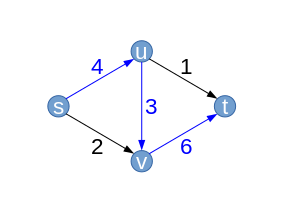
\includegraphics{graph1} 
  \caption{Bild eines Netzwerk-Graphen}
  \label{fig:Graph1}
\end{figure}

\subsection{Algorithmus von Ford und Fulkerson}
Der Ford und Fulkerson Algorithmus errechnet mittels einem Netzwerk $(G,u,s,t)$ den maximalen Fluss $f$.\\ \\Input: Netzwerk $(G, u, s, t)$.\\Output: Maximaler Fluss $f$.\\ \\
Schritt 1: Setzen Sie $f(e) = 0$ für alle Kanten $e \subseteq E$.\\ \\Schritt 2: Bestimmen Sie $Gf$ und $uf (e)$.\\ \\Schritt 3: Konstruieren Sie einen einfachen $(s, t)$-Weg $p$ in $Gf$ . Falls keiner existiert:
STOPP.\\ \\Schritt 4: Verändern Sie den Fluss $f$ entlang des Wegs $p$ um $Y := mine \subseteq p uf (e)$.\\ \\Schritt 5: Gehen Sie zu Schritt 2


\subsection{Algorithmus von Edmonds und Karp}
Beschreibung und Erläuterung des Edmonds und Karp Algorithmus

\subsection{Algorithmus von Dinic}
Beschreibung und Erläuterung des Algorithmus von Dinic


\section{Der Inhalt}
\label{Inhalt}
Kriterien der Evaluierung, Vorstellung des Testaufbaus
\section{Experimente}
\label{Experimente}
Auflistung Test welche Daten benutzen wir und was wir damit erreichen wollen?
\subsection{Laufzeitvergleich}
Vergleich der Test Ergebnisse

\subsection{Anwendungszenarien der jeweiligen Algorithmen}
Die Ergebnisse also wann welcher anzuwenden ist

\section{Stand der Technik (Related Work)}
\label{Related Work}
\subsection{Algorithmen und Datenstrukturen Springer Verlag}
Text text text text. Text text text text. Text text text text. Text text text text. Text text text text. Text text text text. Text text text text. Text text text text. 
\subsection{Graphentheoretische Konzepte und Algorithmen Vieweg und Teubner}
Text text text text. Text text text text. Text text text text. Text text text text. Text text text text. Text text text text. 
\section{Zusammenfassung}
\label{Zusammenfassung}
Text text text text. Text text text text. Text text text text. Text text text text. Text text text text. Text text text text. 

\subsection{Ausblick}
Erweiterung des Algorithmus von Dinic und Bottleneck erkennen.

\bibliography{test}
\bibliographystyle{plainnat} 

\end{document}
